\chapter{Theoretical Background}
%\thispagestyle{empty}% no page number in chapter title page


\section{Bayesian neural network}
In this chapter, a brief review on theory of Bayesian neural network is given. Because calculating the exact posterior distribution over the parameters of large and complex neural network is intractable, proper techniques to perform approximate inference are required, which can be categorized into two mainstreams, variational inference(VI) and Markov Chain Monte Carlo(MCMC). However, since larger dataset and more complex neural network are popular and working pretty well nowadays, traditional approximate inference techniques are difficult to scale to large dataset and complex advanced architectures. Therefore modern approximate inference needs to be adopted. In this section, we introduce and evaluate two modern approximate inference methods for neural network, which are dropout variational inference\cite{gal2016dropout} and scalable Laplace approximation\cite{ritter2018scalable}. Additionally, we introduce concrete dropout \cite{gal2017concrete} to improve uncertainty estimation by learning dropout rate from data instead of tuning them by hand before training.

\subsection{Introduction}

Let $\mathcal{D}$ denote an observable dataset consisting of a set of input and output pairs, that is $\mathcal{D} = \{\mathbf{X}, \mathbf{Y}\} = \{(x_{i}, y_{i})_{i=1}^{N}\}$, where $x_{i}\in\mathbb{R}^{D}$ and $y_{i}\in\mathbb{Y}$, $\mathbb{Y}$ is set of labels, and $f^{\boldsymbol{\omega}}$ denote one parametric model which is in our case neural network with {\boldmath{$\omega$}} its parameters which are weights $W_{1:L}$ and biases $b_{1:L}$ for $L$ layers.

In supervised learning, our goal is to learn a distribution of output conditioned on input, $p(\mathbf{y}|\mathbf{x})$ that can explain the underlying data distribution based on the observables $\mathcal{D}$ which are samples drawn from the underlying data distribution. Then this learned model can be used to make predictions on unobservable data samples under the same data distribution. In classification where output is label represented by discrete integer, the likelihood function is defined based on parametric model, which is softmax score:
\begin{equation}
p(y = d|\mathbf{x}, \boldsymbol{\omega}) = \frac{exp(f^{\boldsymbol{\omega}}_{d})}{\sum_{d'}exp(f^{\boldsymbol{\omega}}_{d'})}  \label{2.1}
\end{equation}
where $d$ is possible class of random variable $y$, and $f^w_d$ represents the probability that class $d$ is assigned to $y$.  

In regression case, the likelihood is Gaussian:

\begin{equation}
p(\mathbf{y}|\mathbf{x}, \boldsymbol{\omega}) = \mathcal{N}(\mathbf{x}; f^{\boldsymbol{\omega}}(\mathbf{x}), \tau^{-1}\textbf{I}) 
\label{2.2}
\end{equation}

with model precision $\tau$, which represents the inverse of noise level of the outputs.

As mentioned above, learning aims to find model(s) which is parameterized by a set of parameters that can explain the data well, which means the likelihood should be maximized w.r.t. model parameters over the observables. On the other hand, some prior constraints are imposed on the model via prior distribution of the model parameters $p(\boldsymbol{\omega})$. The probability distribution of model parameters is updated from prior distribution into posterior distribution after observing training dataset $\mathcal{D}$ via Bayes' theorem:

\begin{equation}
p(\boldsymbol{\omega}|\mathbf{X}, \mathbf{Y}) = \frac{p(\mathbf{Y}|\mathbf{X}, \boldsymbol{\omega})p(\boldsymbol{\omega})}{p(\mathbf{Y}|\mathbf{X})}
\label{2.3}
\end{equation}

where $p(\mathbf{Y}| \mathbf{X}) = \int p(\mathbf{Y}| \mathbf{X}, \boldsymbol{\omega})p(\boldsymbol{\omega})d\boldsymbol{\omega}$ is so called model evidence or marginal likelihood, whose integration is always intractable.

After obtaining posterior distribution over model parameters, we can make predictions by marginalizing the likelihood of unseen input points such as $x^{\star}$ over model parameters, which leads to predictive distribution over output:

\begin{equation}
p(y^{\star}|x^{\star}, \mathcal D) = \int p(y^{\star}|x^{\star}, \boldsymbol{\omega})p(\boldsymbol{\omega}|\mathcal D)d\boldsymbol{\omega}
\label{2.4}
\end{equation}

Pointing out the difference between deterministic neural network and Bayesian neural network can help understanding the mechanism of Bayesian neural network better. In Fig.\ref{fig:dnn_bnn}, we use graphical model to express these two kinds of neural network, in which solid point denotes deterministic variable, and circle denotes random variable, while the shaded circle denotes observed random variable. Plate notation denotes $N$ observed data pairs $(\bld x, \bld y)$. Fig.\ref{fig:dnn_bnn} demonstrates that parameters $\boldsymbol{\omega}$ in deterministic is normal variable which is a point estimate done by Maximum a posterior method:

\begin{equation}
\boldsymbol{\omega^{\star}} = \underset{\bld \omega}{argmax}\{p(\mathbf{Y}|\mathbf{X}, \boldsymbol{\omega})\}\label{2.5}
\end{equation}

On the other hand, in Bayesian neural network, the model parameter $\boldsymbol{\omega}$ is random variable with distribution parameterized by $\theta$. To note that for explanation of concept here, we do not make any assumption on the function parameterized by $\theta$, which means it can be arbitrary function. This distribution over model parameters can be inferred based on Bayes' rule in Eq.\ref{2.3}. However, for model with large number of parameters, it's hard to compute the model evidence (denominator of r.h.s of Eq.\ref{2.3}) with integration tractably. Approximation needs to be employed to solve this problem. It's worth noting that if we choose the approximate distribution to be delta function, $q_{\theta}(\bld \omega) = \delta(\bld \omega - \theta)$, Bayesian neural network is recovered into deterministic neural network. Because the computation of model evidence $p(\mathbf{Y}|\mathbf{X})$ is always intractable in complex model and large dataset, we need to resort to approximate inference, which will briefly be introduced in next section.


\begin{figure}[H]
	\begin{center}
		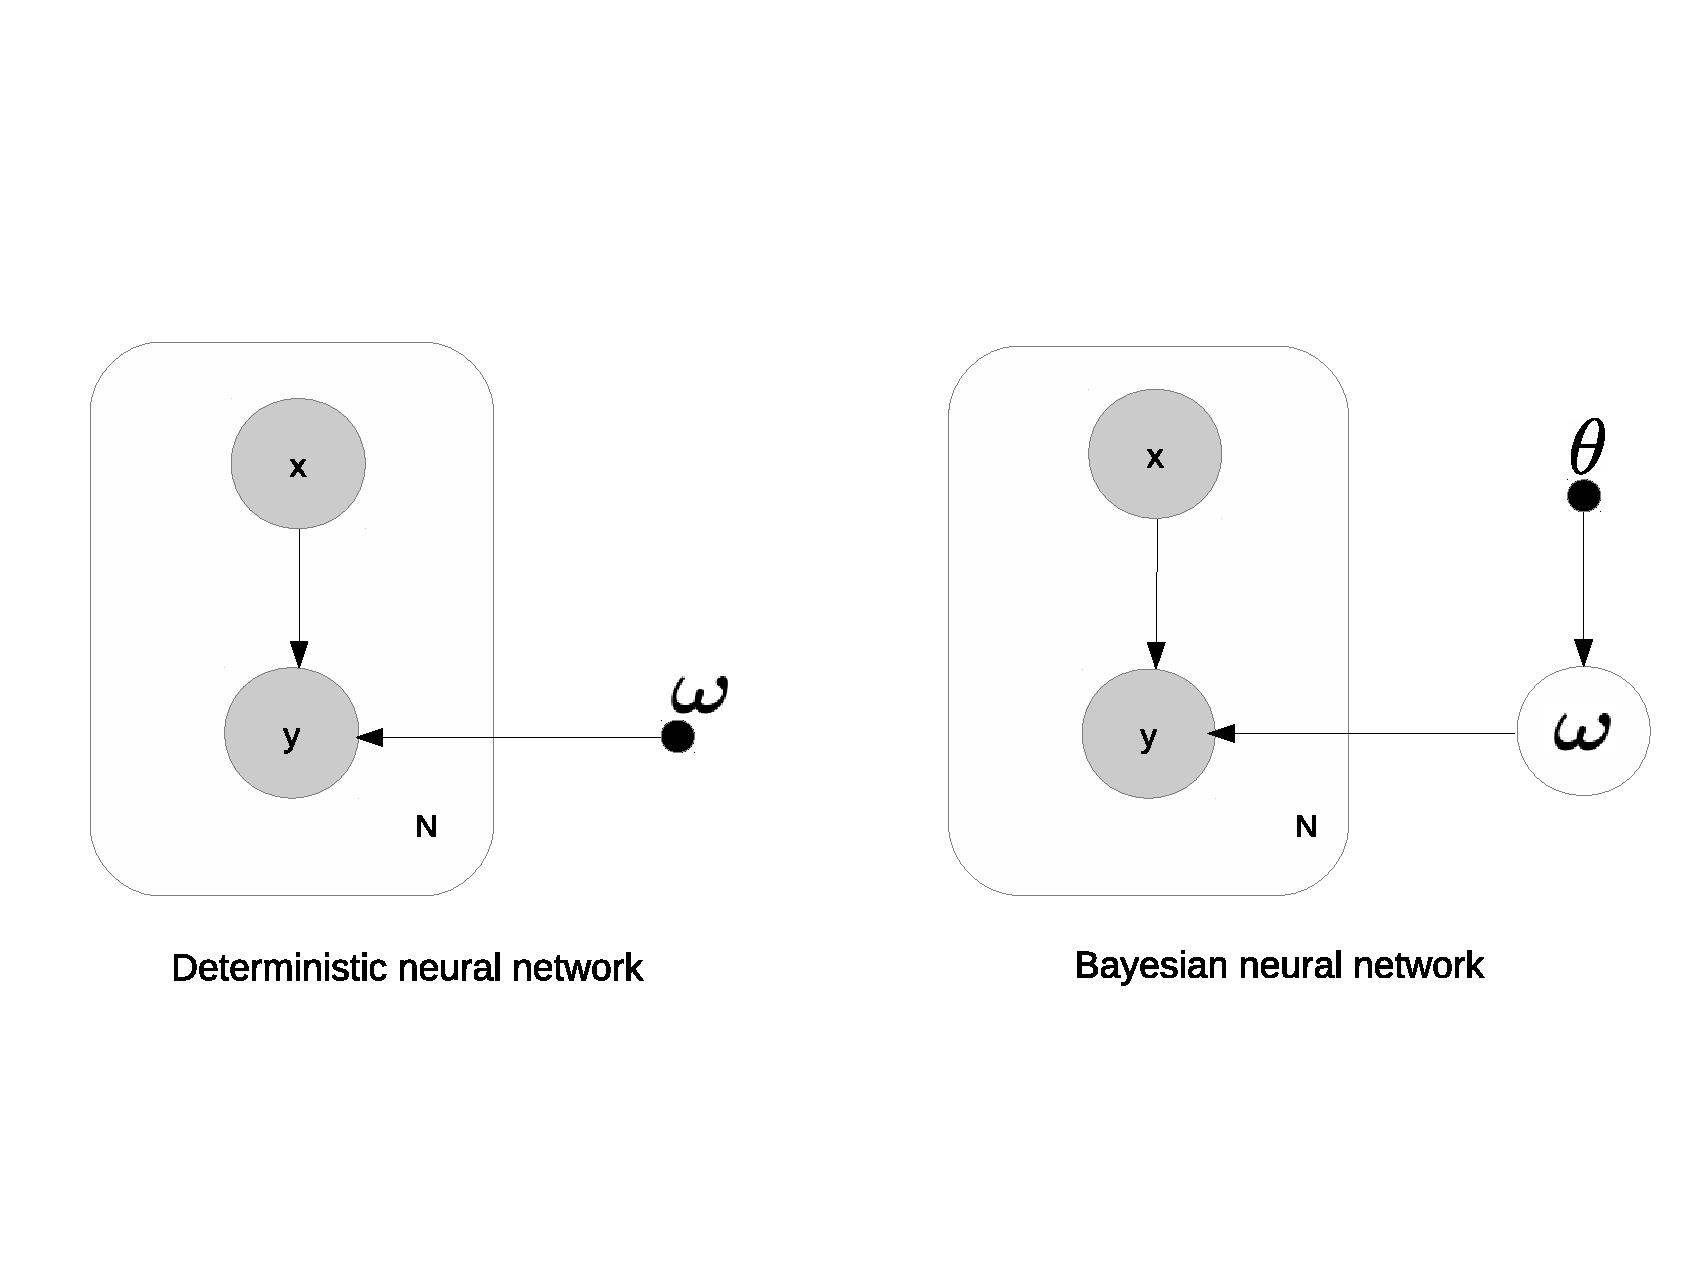
\includegraphics[height=9.1cm, width=12cm]{dnn_bnn}
		\caption{Difference between parameter estimation of deterministic neural network and Bayesian neural network.}		
		\label{fig:dnn_bnn}
	\end{center}
\end{figure}

\subsection{Dropout variational inference}
\subsubsection{Introduction}
Variational inference cast inference into optimization by minimizing the Kullbach-Leibler divergence between approximate posterior distribution and the real posterior distribution. However, there is no analytical definition of this KL divergence because the real posterior distribution is unknown. We can derive a lower bound which is also called evidence lower bound($ELBO$) which bounds the log marginal likelihood with Jensen's inequality. And from that we know that marginal likelihood is the sum of $ELBO$ and KL divergence between approximate posterior and real posterior. The derivation is given in the following:
\begin{equation}\label{2.6}	
\begin{aligned}
\log(p(\bld{Y}|\bld{X})) & = \log(\int p(\bld{Y}| \bld{X}, \bld{\omega})  p(\bld{\omega})d\bld{\omega}) \\	 
& = \log(\int{q_{\theta}(\bld{\omega}) \frac{p(\bld{Y}| \boldsymbol{X}, \bld{\omega}) p(\bld{\omega})}{q_{\theta}(\bld{\omega})}d\bld{\omega}}) \\
& \geq \int q_{\theta}(\bld{\omega}) \log( \frac{p(\bld{Y}| \bld{X}, \bld{\omega}) p(\bld{\omega})}{q_{\theta}(\bld{\omega})}) d\bld{\omega} \\
& = \mathbb E_{q_{\theta}(\bld{\omega})}[\log(p(\bld{Y}| \bld{X}, \bld{\omega}))] -  KL(q_{\theta}(\bld{\omega}||p(\bld{\omega})))\\
& = ELBO
\end{aligned}
\end{equation}

where $p(\bld Y| \bld X)$ is the likelihood, $p(\bld \omega)$ is the prior distribution over model parameters, $q_{\theta}(\bld \omega)$ is the approximate posterior distribution over parameters which is parameterized by $\theta$.

We can get log$(p(\bld Y) | \bld X)$ by calculating the sum of $ELBO$ and KL divergence between approximate posterior $q_{\theta}(\bld \omega)$ and real posterior $p(\bld \omega | \bld X, \bld Y)$:

\begin{equation}\label{2.7}	
\begin{aligned}
& ELBO + KL(q_{\theta}(\bld{\omega}) || p(\bld{\omega}|\bld{X}, \bld{Y})) \\ 
& = \int q_{\theta}(\bld{\omega}) \log( \frac{p(\bld{Y}| \boldsymbol{X}, \bld{\omega}) p(\bld{\omega})}{q_{\theta}(\bld{\omega})}) d\bld{\omega} + \int q_{\theta}(\bld{\omega}) \log(\frac{q_{\theta}(\bld{\omega})}{p(\bld{\omega}|\bld{X}, \bld{Y})}) d\bld{\omega} \\
& = \int q_{\theta}(\bld{\omega}) \log(p(\bld{Y} | \bld{X}))d\bld{\omega}\\
& = log(p(\bld{Y}|\bld{X})) 
\end{aligned}
\end{equation}

When we maximize the $ELBO$ w.r.t the parameter of approximate posterior $\theta$, which is also called \textbf{variational parameter}. We use these two terms interchangeably in the following. It's equivalent to minimizing the KL divergence because the log marginal likelihood is not a function of $\theta$. Then we have a well-defined objective which is the $ELBO$, in which the first term is called expected log likelihood which ensures the model can explain the data well and the second term is called regularization term which ensures the approximate posterior does not deviate too far from the prior distribution.
Now the inference problem has been cast into an optimization problem:

\begin{equation}\label{2.8}	
\begin{aligned}
\theta^{\star} = \underset{\theta}{argmin} \{KL(q_{\theta}(\bld \omega)||p(\bld \omega | \bld X, \bld Y))\}
\end{aligned}
\end{equation}

which is equivalent to 

\begin{equation}\label{2.9}	
\begin{aligned}
\theta^{\star} = \underset{\theta}{argmax}\{ELBO\}
\end{aligned}
\end{equation}

However, there are still some difficulties if we want to solve this optimization with this objective. The first one is to deal with large size dataset, which induces large computation in the expected log likelihood term. \cite{graves2011practical} shows that this can solved by data sub-sampling which is also called stochastic optimization. Another one is that we need to obtain the derivatives of $ELBO$ w.r.t. approximate parameter $\theta$. Since the model parameters are samples from approximate distribution, good estimator for the derivatives is required which will be introduced in next subsection. 

\subsubsection{Dropout variational inference}
\paragraph{Dropout\cite{srivastava2014dropout}} is originally introduced as regularization approach in training deep neural network which can improve the generalization performance. Although the author said this idea is inspired from human beings sexual reproduction, there are different interpretations trying to explain why it can work such as ensemble perspective and Bayesian perspective. In this subsection, the Bayesian interpretation of dropout is introduced and used for improving the uncertainty estimation of neural network. 

The mechanism of dropout is straightforward, each units of specific layer is multiplied by a random variable under Bernoulli distribution with $1-p$ as its parameter, where $p$ is the so-called dropout rate. In each iteration of training, dropout is turned on, which means each unit is multiplied by the sample drawn from Bernoulli distribution in forward propagation which is kept in derivatives back propagation during current iteration. In testing, the sampling phase is turned off, only one forward propagation is needed to obtain predictions. Normally, in order to avoid rescaling weights in testing, which is used to keep the output magnitudes in the same scale when dropout is off, rescaling of the output of dropout is always done in training. In Fig.\ref{fig:dropout}, there are two figures showing how dropout is turned on and off. 
\begin{figure}[H]
	\begin{center}
		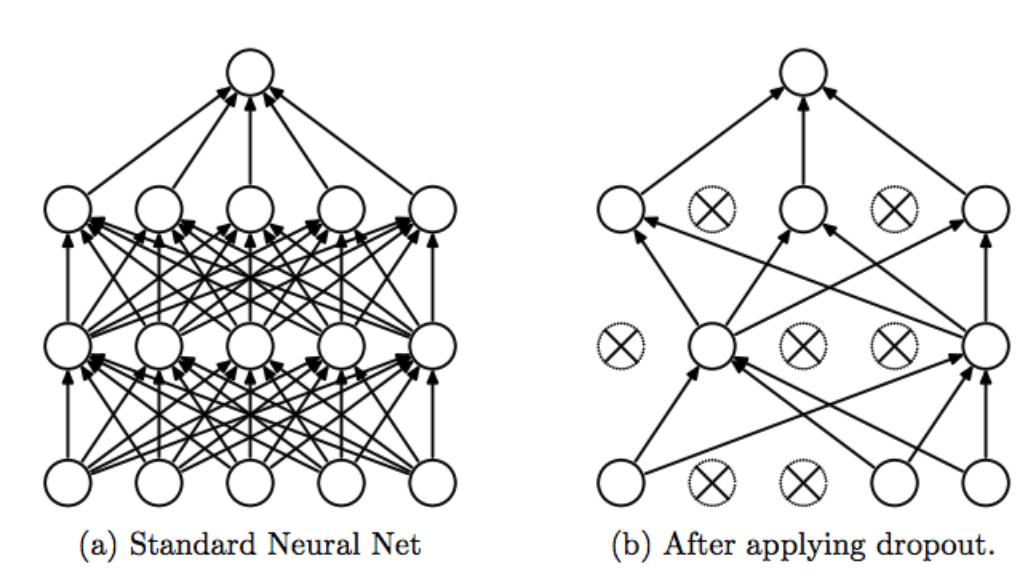
\includegraphics[height=7cm, width=13cm]{dropout}
		\caption{How dropout works\cite{srivastava2014dropout}.}		
		\label{fig:dropout}
	\end{center}
\end{figure}


\paragraph{Bayesian interpretation of dropout:}
In VI, the goal is to minimize the KL divergence between approximate distribution and the real posterior distribution over the model parameters. This objective is equivalent to maximization of evidence lower bound($ELBO$). When dropout is interpreted in Bayesian way, the distribution over hidden units is reformulated as distribution over weight matrices. The training objectives of neural network with dropout is proved to be similar as the $ELBO$ of Bayesian neural network with Bernoulli distribution factorized over the input dimension of weight matrix. In the following, we will explain this interpretation including following key factors: \textbf{approximate distribution}, \textbf{training objective}, \textbf{marginalization in testing} by using one simple example in {classification} case in Fig.\ref{fig:dropout_inference}, in which we define the hidden layer as the first layer and output layer as the second layer and assume a fully factorized Gaussian prior over parameters.


\begin{figure}[h!]
	%\begin{center}
	\centering
	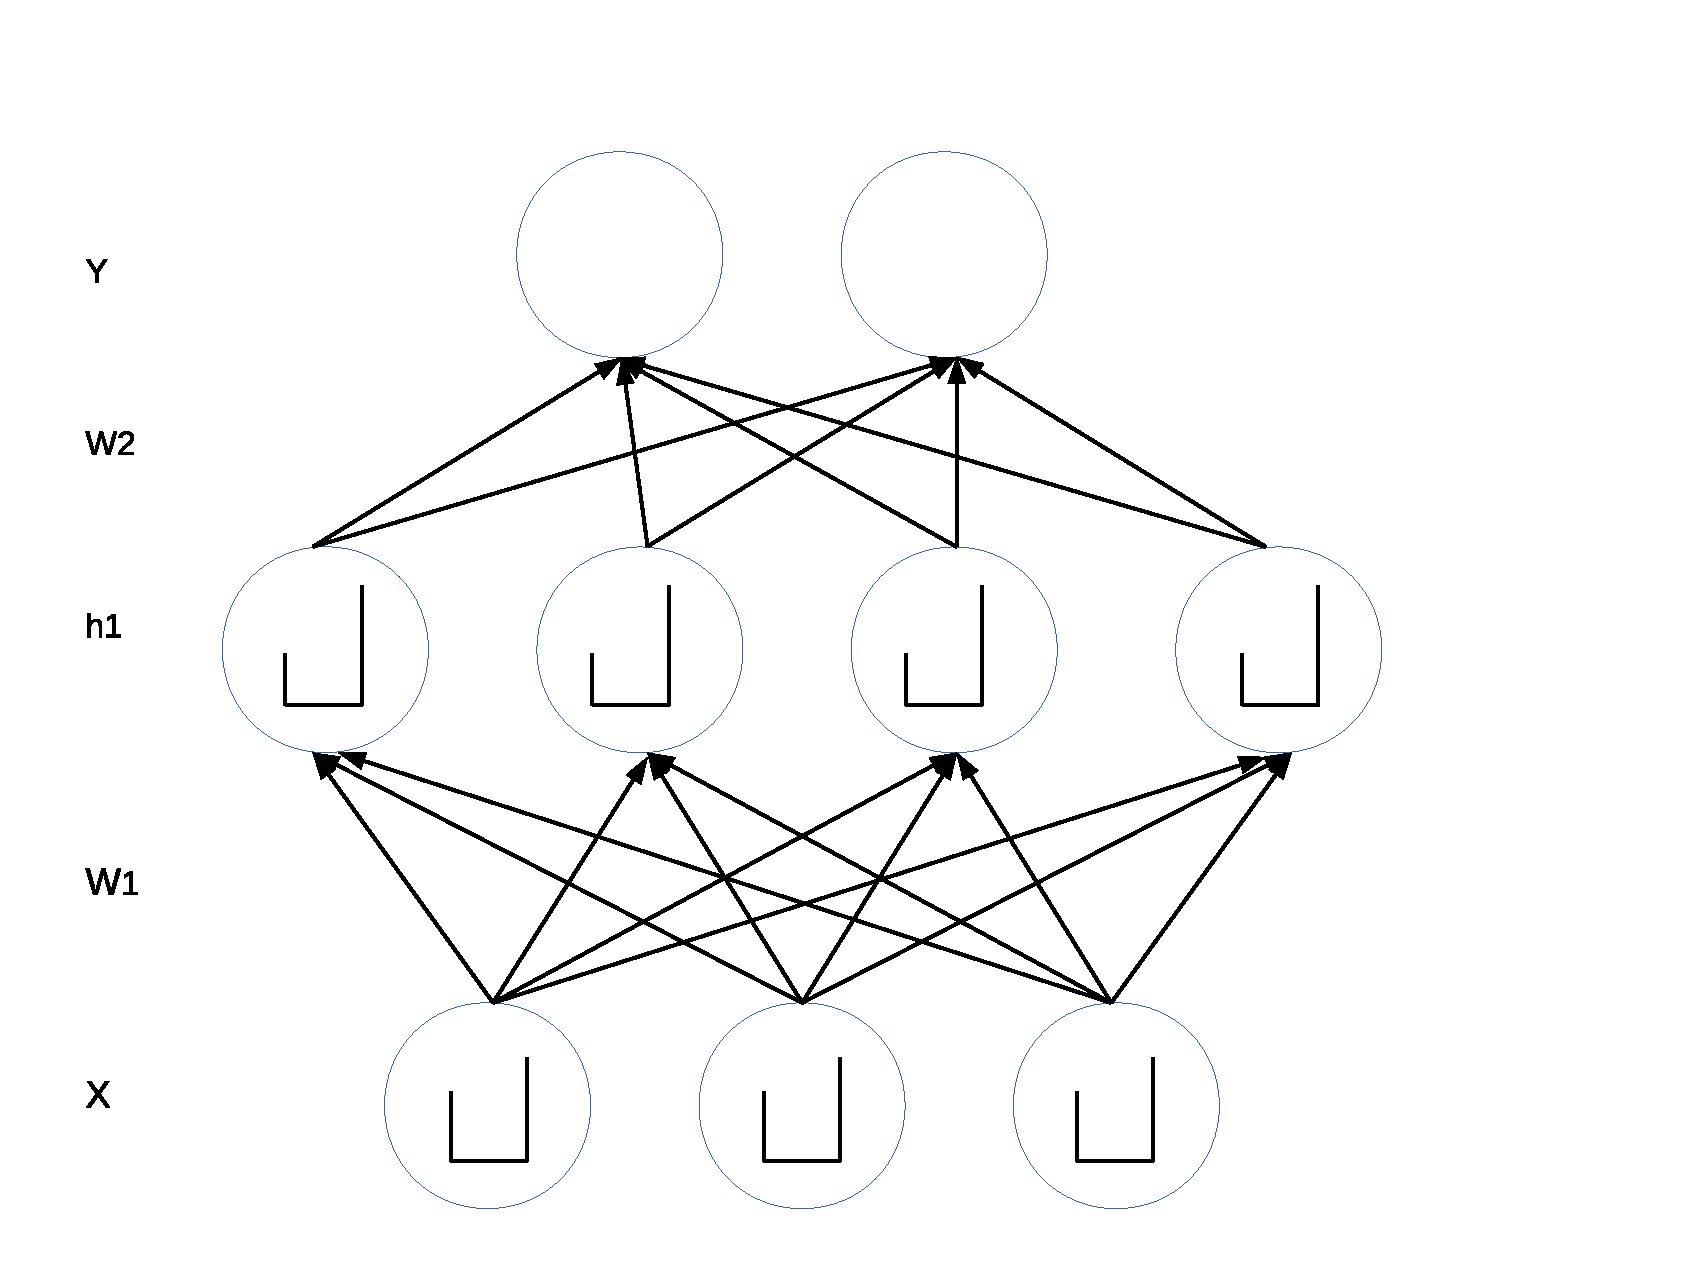
\includegraphics[height=8cm, width=11cm]{dropout_inference}
	\caption{An example of two layer neural network with dropout, a Bernoulli random variable is imposed on each unit of input layer and hidden layer.}		
	\label{fig:dropout_inference}
	%\end{center}
\end{figure}


\subparagraph{Approximate distribution:}
Let's denote $\bld y\in \mathbb R ^{m \times D_{2}}$ as output, $\bld x \in \mathbb R^{m \times D_{0}}$ as input, $\bld h_{1} \in \mathbb R^{D_{1}}$ as the response of hidden layer, where $m$ represents number of data instances, $D_{i}$ is dimensionality of $i$-th layer, where $0$-th layer represents input layer and $i \in \{1,..,L\}$, $L=2$ in this example. Further we define $\bld \omega = \{ (\bld W_{i})_{i=1}^{L}  \}$ as model parameters, and $\bld \epsilon_{i} \in \mathbb R^{D_{i-1}}$ as the Bernoulli distributed random vector parameterized by $\bld p_{i} \in \mathbb R^{D_{i-1}}$, for $i$-th layer. In normal dropout, elements in vector $\bld p_{i}$ have same values $p_{i}$, which means that there is one keep rate or ($1-$dropout rate) for each layer. In the following, we will use $\bld p_{i}$ and $p_{i}$ interchangeably depending on the context if there is no special specification. To note that since weight matrix is treated as random variable, we use $\bld M_{i} \in \mathbb R^{D_{i-1} \times D_{i}}$ to denote position of non-zero element in Bernoulli distribution for $\bld W_{i}$. To note that bias $\bld b_{i} \in \mathbb R^{D_{i}}$ is absorbed into $W_{i}$ by appending a new row at the end of weight matrix and 1 at the end of each data input vector, which is also called homogeneous coordinate. We also assume that approximate weight distribution is factorized over layer, which yields
\[
q_{\theta}(\bld \omega) = \prod_{i=1}^{L}q_{\theta}(\bld W_{i}). 
\]

To start with the formulation of dropout, we model likelihood of output conditioned on input with softmax scores of neural network in classification case:
\begin{equation}
\begin{aligned} \label{dropout_form}
p(\bld y| \bld x, \bld \omega) & = \sigma((\bld h_{1} \odot \bld \epsilon_{2}) \bld M_{2})\\
& = \sigma(\bld h_{1} (diag(\bld \epsilon_{2}) \bld M_{2})) \\
& = \sigma(\bld h_{1} \bld W_{2}) \\
& = \sigma(\phi(\bld x (diag(\bld \epsilon_{1}) \bld M_{1})+ \bld b_{1}) \bld W_{2}) \\
& = \sigma(\phi(\bld x \bld W_{1})\bld W_{2})
\end{aligned}
\end{equation}

where $\odot$ is Hadamard product(element-wise product), $\sigma(a_{j}) = \frac{exp({a_{j}})}{\sum_{k}exp({a^{k}})}$ is softmax function, $\phi(\cdot)$ is element-wise non-linear activation function such as rectified unit function.

From the equation above, we have 

\[
\bld W_{i} = g(\bld M_{i}, \bld \epsilon_{i})= diag(\bld \epsilon_{i}) \bld M_{i} 
\]
\[ 
\text{ with } \bld \epsilon_{i} \sim p(\bld \epsilon_{i}) = Bernoulli(\bld p_{i}) 
\]

which means weight matrix $\bld W_{i}$ is a random variable whose probability density function is parameterized by $\bld p_{i}$ and $\bld M_{i}$, which are denoted by $\theta = \{ (\bld M_{i}, \bld p_{i})_{i=1}^{L} \}$ in Eq.\ref{2.8}, where $i = {1,..,L}$ denotes $i$-th layer of the network, and $L = 2$ in this example. 
The expression of approximate posterior distribution is not obvious, but we can define the its form as 

\begin{equation}
\begin{aligned} \label{appro_dist_form}
q_{\theta}(\bld \omega) &= \prod_{i=1}^{L} q_{\theta}(\bld W_{i})\\
&= \prod_{i=1}^{L}\int q_{\theta}(\bld W_{i} | \bld \epsilon_{i})p(\bld \epsilon_{i}) d\bld \epsilon_{i} 
\end{aligned}
\end{equation}
with

\begin{equation}
\begin{aligned} \label{appro_cond_dist_form}
q_{\theta}(\bld W_{i}|\bld \epsilon) &= \delta(\bld W_{i} - g(\bld M_{i}, \bld \epsilon_{i}))  \\
& = \delta(\bld W_{i} - diag(\bld \epsilon_{i})\bld M_{i})
\end{aligned}
\end{equation}

As we can see, the approximate posterior distribution over the parameter matrix puts a same Bernoulli distribution over the input dimension of parameter matrix, which is the row dimension in this example.  Meanwhile each element of the same row is multiplied with same realization of the random variable but with different non-zero position, which is corresponding to different expectation of each row element and thus induces correlations between row elements. To make this definition more clear, based on the computation of expectation and variance of Bernoulli distribution, we can write down the first and second moment of the approximate distributed random variables in the following:

\begin{equation}
\begin{aligned} \label{appr_expectation}
\mathbb E_{q_{\theta}}(\bld W_{i}) & = \bld M_{i} \odot \bld P_{i}
\end{aligned}
\end{equation}

where $\bld P_{i} = [\bld p_{i}, ..., \bld p_{i}] \in \mathbb R^{D_{i-1} \times D_{i}}$.

Covariance matrix of parameter matrix is:

\begin{equation}
\begin{aligned} \label{appr_covariance}
\big[Cov_{q_{\theta}}(vec(\bld W_{i}))\big]_{jk}   = \mathbbm{1} \big[l=m\big] m^{i}_{lq}*m^{i}_{mn}*p_{i}*(1-p_{i})
\end{aligned}
\end{equation}

where 
\[ j = l*D_{i-1} + q\],
\[ k = m*D_{i-1} + n\],
which is the linear mapping between element index before and after matrix vectorization. $m^{i}_{lq}$ is the element of $l$-th row and $q$-th column in matrix $\bld M_{i}$, which applies to $m^{i}_{mn}$ as well. $\mathbbm 1 \big[i=j\big]$ denotes indicator function, which is equal to 1 only when $i$ is equal to $j$ and otherwise 0. Because $vec(\cdot)$ operation converts matrix $\bld W_{i} \in \mathbb R^{D_{i-1} \times D_{i}}$ into column vector $ vec(\bld W_{i}) \in \mathbb R^{D_{i-1}D_{i} \times 1}$ by stacking the columns of matrix on top of one another. Then it's easy to see that covariance matrix $Cov_{q_{\theta}}(vec(\bld W_{i})) \in \mathbb R^{D_{i-1}D_{i} \times D_{i-1}D_{i}} $. 

From Eq.\ref{appr_covariance}, we can see that the entire covariance matrix is consisting of $D_{i} \ast D_{i}$ diagonal sub-matrices whose dimensionality are $D_{i-1} \times D_{i-1}$.
When observing covariance matrix of parameter matrix $\bld W_{i}$ w.r.t. approximate posterior distribution $q_{\theta}({\bld W_{i}})$, we know that samples of row vectors in weight matrix are drawn independently and thus covariance between rows are zero. On the other hand, samples for different weights in the same row are drawn at the same time because they are multiplied by the same realization of $\epsilon_{i}$, from which covariances between weights within the same row are induced. Therefore, by fitting this approximate distribution to the real posterior distribution weights within the same row can be learned. This means that the approximate distribution family have more flexibility to approximate the real posterior distribution when compared with other common approximate posterior distribution family that assumes distribution for each parameter is independent such as fully factorized Gaussian.


\subparagraph{Training objective:} Up to now, we have only analyzed the approximate distribution of dropout inference. As is mentioned in introduction section of this chapter, we know that we perform optimization of $ELBO$ w.r.t. the approximate distribution parameters, in order to obtain a good approximation to the true posterior distribution over parameters, which we can use in testing to obtain more reliable uncertainty estimation. In the following, we will show that training a neural network with dropout is equivalent to optimizing the $ELBO$ w.r.t. variational parameters.

At first, let's define the training objective of neural network with dropout, which is cross entropy between predictive distribution and target distribution plus L2 regularization:

\begin{equation}
\begin{aligned} \label{dropout_loss}
L_{dropout}   = \sum_{i=1}^{N}\big[-log(p(\bld y_{i}| \bld x_{i}, \bld \omega))\big] + \lambda(\sum_{i=1}^{L} ||\bld W_{i}||^{2})
\end{aligned}
\end{equation}

where $N$ represents the size of entire dataset, $\lambda$ is L2 regularization coefficient. We want to maximize the likelihood over the entire dataset w.r.t. the model parameter $\bld \omega$, which is known as maximum likelihood estimation. Equipped with L2 regularization and Gaussian prior over parameters, we can obtain a max-a-posterior estimation by minimizing Eq.\ref{dropout_loss}. 

Normally we use gradient descent to tune our parameters in training, which requires first derivative of objective w.r.t. model parameters $\bld \omega$. Since nowadays large size of dataset is ubiquitous, which means $N$ in Eq.\ref{dropout_loss} is too large, we could not obtain exact gradient of entire batch with efficient computation. Therefore we use data of mini-batch to estimate gradient, which is so called stochastic gradient descent(SGD). Apart from making computation tractable, noise of gradient estimation in each mini-batch is helpful for optimization procedure to escape the poor local minimum. The expression of gradients required in each iteration of SGD is given in the following:

\begin{equation}
\begin{aligned} \label{dropout_grad}
\frac{\partial L_{dropout}}{\partial \bld \omega} &=\frac{N}{K}\sum_{i \in S}\big[-\frac{\partial log(p(\bld y_{i}| \bld x_{i}, \bld \omega))}{\partial \bld \omega}\big] + \lambda\frac{\partial (\sum_{i=1}^{L} ||\bld W_{i}||^{2})}{\partial \bld \omega}
\end{aligned}
\end{equation}

where $S$ is one random subset of entire dataset, and $|S| = K$.

On the other hand, let's have a look at $ELBO$ in Eq.\ref{2.6}, if we want to maximize $ELBO$, which is equivalent to minimize negative $ELBO$ w.r.t. the variational parameter $\theta$, with SGD. The gradients are computed with the following expression:

\begin{equation}
\begin{aligned} \label{elbo_grad}
\frac{\partial (-ELBO)}{\partial \theta} &=\frac{N}{K}\sum_{i \in S}\big[-\frac{\partial \mathbb E_{q_{\theta}(\bld \omega)} \big[log(p(\bld y_{i}| \bld x_{i}, \bld \omega))\big]}{\partial \theta}\big] + \frac{\partial KL(q_{\theta}(\bld \omega)||p(\bld \omega))}{\partial \theta}
\end{aligned}
\end{equation}

In order to calculate two terms in Eq.\ref{elbo_grad}, we need to introduce one technique called re-parameterization trick\cite{kingma2013auto} for the first term and one condition called KL condition\cite{gal2016uncertainty} for the second term in the following.

\subparagraph{Re-parameterization trick:} when we take a close look at the first term in Eq.\ref{elbo_grad}, we know that we need to compute the gradients of expectation w.r.t. the parameters of distribution to which this expectation is subject. That means, we need to estimate the gradients of those parameters because our objective is generated from these parameters randomly. Fortunately, there are different approaches to estimate the gradients of this kind of parameters such as score function or REINFORCE estimator\cite{williams1992simple}, re-parameterization trick \cite{kingma2013auto} and so on. As is stated in \cite{kingma2013auto}, re-parameterization trick has lower variance than score function estimator and is also unbiased. Let's have a quick recap of this technique and see it's already a built-in part in neural network with dropout.

To identify the problem, we can write a more general form of calculus we want to solve in the following:

\begin{equation}
\begin{aligned} \label{repa}
I(\theta) = \frac{\partial}{\partial \theta} \mathbb E_{p_{\theta}(x)} \big[ f(x)\big]= \frac{\partial}{\partial \theta} \int f(x) p_{\theta}(x) dx
\end{aligned}
\end{equation} 

Assume that $p_{\theta}(x)$ can be re-parameterized as $p(\epsilon)$ which is a parameter-free distribution such that random variable $x$ can be generated from a deterministic differentiable function with $\theta$ and $\epsilon$ as arguments, that is

\[
x = g(\theta, \epsilon)  \text{ with } \epsilon \sim p(\epsilon)
\]

Then we can derive the estimator of the gradients w.r.t. distribution parameters $\theta$ with $p(x|\epsilon) = \delta(x-g(\theta,\epsilon))$:
\begin{equation}
\begin{aligned} \label{repa1}
I'(\theta) &= \frac{\partial}{\partial \theta} \int f(x) p_{\theta}(x) dx \\
&= \frac{\partial}{\partial \theta} \int f(x)(\int p_{\theta}(x|\epsilon)p(\epsilon)d\epsilon) dx \\
&= \frac{\partial}{\partial \theta} \int (\int f(x) p_{\theta}(x|\epsilon)dx) p(\epsilon) d\epsilon \\
&= \frac{\partial}{\partial \theta} \int (\int f(x)\delta(x-g(\theta,\epsilon))dx) p(\epsilon) d\epsilon \\ 
&= \frac{\partial}{\partial \theta} \int f(g(\epsilon, \theta)) p(\epsilon) d\epsilon \\
&= \int \frac{\partial}{\partial \theta} f(g(\epsilon, \theta)) p(\epsilon) d\epsilon \\
&= \int f'(g(\epsilon, \theta))\frac{\partial}{\partial \theta}g(\theta, \epsilon) p(\epsilon) d\epsilon \\
&= \mathbb E_{p(\epsilon)}\big[ f'(g(\epsilon, \theta))\frac{\partial}{\partial \theta}g(\theta, \epsilon)\big] 
\end{aligned}
\end{equation} 
From practical point of view, the expectation of last line in expression Eq.\ref{repa1} can be approximated with Monte Carlo integration. In dropout inference, we know that if we fix the dropout rate to $1- p_{i}$ in Eq.\ref{appro_cond_dist_form} during training. Then $\bld \epsilon_{i}$ in Eq.\ref{appro_cond_dist_form} is a parameter free random variable and $g(\cdot)$ is a differentiable function w.r.t. its input argument $\bld M_{i}$. Now the variational parameter $\theta$ only contains $\{(\bld M_{i})_{i=1}^{L} \}$, which are exactly the weights to be learned in training neural network with dropout. As a consequence, if we estimate the gradient of $ELBO$ w.r.t. $\{(\bld M_{i})_{i=1}^{L}\}$, which is the first term in Eq.\ref{elbo_grad}, it's equivalent to calculate the gradient of dropout loss w.r.t. model parameters $\bld \omega$ which is the first term in Eq.\ref{dropout_grad}.

\subparagraph{KL condition:} The second term in Eq.\ref{elbo_grad} is proved to be equivalent to the second term in Eq.\ref{dropout_grad}
for a large enough number of hidden units when we specify the model prior to be a product of independent Gaussian distributions over each weight with prior length scale $l$, that is:
\[p(\bld \omega) = \prod_{i=1}^{L}(p(\bld W_{i})) \]
with
\[
p(vec(\bld W_{i})) = \mathcal N(0, l^{-2}\bld I_{D_{i-1} D_{i}})
\]

To establish this condition, we need to make a approximation of the approximate posterior distribution $q_{\theta}(\bld \omega)$ in Eq.\ref{appro_dist_form}, where we approximate $q_{\theta}(\bld W_{i}|\bld \epsilon_{i})$ in Eq.\ref{appro_cond_dist_form} as a narrow Gaussian with a very small standard deviation. As we know, $q_{\theta}(\bld W_{i})$ factorizes over each row of the weight matrix. Then that means $q_{\theta}(\bld \omega)$ is a mixture of two Gaussians with small standard deviations, and one component fixed at zero:
\begin{equation}\label{appro_dist_guassian}
\begin{aligned}
q_{\theta}(\bld \omega) &= \prod_{i=1}^{L}q_{\theta}(\bld W_{i}) \\
&=\prod_{i=1}^{L}\prod_{j=1}^{D_{i-1}}q_{\theta}(\textbf{w}_{i,j}) \\
&= \prod_{i=1}^{L}\prod_{j=1}^{D_{i-1}} \big[ p_{i} \mathcal N(\textbf{m}_{i,j},\sigma^{2} \bld I_{D_{i}}) + (1-p_{i})\mathcal N(\bld 0, \sigma^{2} \bld I_{D_{i}})\big]
\end{aligned}
\end{equation}
where $\textbf{w}_{i,j} \in \mathbb R^{D_{i}}$ is the $j$-th row of weight matrix $\bld W_{i}$ and $p_{i}$ is the parameter of Bernoulli distributed random variable of $i$-th layer. With this, the KL divergence between approximate posterior and prior is KL divergence between mixture of Gaussian and a single Gaussian. 
%In order to keep this report as self-contained as possible, we attach 
Reader who has interest can refer to derivation of KL divergence between mixture of Gaussian and single Gaussian in \cite{gal2016uncertainty}. Then we have KL condition in the following:

\begin{equation}
\begin{aligned} \label{kl_condition}
KL(q_{\theta}(\bld \omega) || p(\bld \omega)) \approx \sum_{i=1}^{L} \sum_{j=1}^{D_{i-1}}
\big[
\frac{p_{i}}{2}(l^{2}\bld m_{i,j}^{T} \bld m_{i,j} + D_{i}( \sigma^{2} -\text{log}(\sigma^{2}) -2\text{log} l- 1) - \mathcal H (\bld p_{i}) 
\big] 
\end{aligned} 
\end{equation}
with 
\[
\mathcal H(\bld p_{i}) = D_{i-1}(-p_{i}\text{log}p_{i} - (1-p_{i})\text{log}(1-p_{i}))
\]
for large enough $D_{i}$. If we \textbf{fix dropout rate} in training and compute the gradients of KL divergence w.r.t. variational parameters $\theta = \{(\bld M_{i})_{i=1}^{L} \}$, which is now exactly the same as the model parameters $\bld \omega = \{(\bld W_i)_{i=1}^L\}$. Then the term entropy of dropout rate can be ignored.  We can see that, if we choose $\lambda = \frac{l^{2}p_{i}}{2}$, then it's equivalent to the gradients of regularization term in dropout loss function(cf. Eq.\ref{dropout_grad}):

\begin{equation} 
\begin{aligned}\label{KL_grad}
\frac{\partial KL(q_{\theta}(\bld \omega)||p(\bld \omega))}{\partial \theta} \approx \frac{\partial \sum_{i=1}^{L}\lambda||\bld M_{i}||^{2}}{\partial \theta}
\end{aligned}
\end{equation}

With aforementioned re-parameterization trick and KL condition, we know that the computation of gradients of objective function w.r.t. model parameters in Eq.\ref{dropout_grad} is equivalent to that of negative $ELBO$ w.r.t. variational parameter in Eq.\ref{elbo_grad}. That means, if we train a neural network with dropout, it's equivalent to train a Bayesian neural network with approximate posterior distribution over model parameters defined in Eq.\ref{appro_dist_form}.

\subparagraph{Marginalization in testing:}
After we have obtain the parameters $\theta$ of approximate posterior distribution over model parameters $q_{\theta}(\bld \omega)$, we can marginalize all possible parameters over approximate posterior distribution to get final predictive distribution of output, similar to Eq.\ref{2.4} but now with approximate posterior distribution over model parameter, which has an expression in Eq.\ref{marginalization_test}. Because the integration is hard to evaluate analytically. In practice, we always use Monte Carlo integration:

\begin{equation}
\begin{aligned} \label{marginalization_test}
p(\bld y^{\star}| \bld x^{\star},\mathcal D) &= \int p(\bld y^{\star} | \bld x^{\star}, \bld \omega) p(\bld \omega |\mathcal D)d\bld \omega \\
&\approx \int p(\bld y^{\star} | \bld x^{\star}, \bld \omega) q_{\theta}(\bld \omega)d\bld \omega \\
&\approx \frac{1}{K}\sum_{i=1}^{K} p(\bld y^{\star} | \bld x^{\star}, \bld{\hat \omega_{i}}) 
\end{aligned}
\end{equation}

where $\bld \omega \sim q_{\theta}(\bld \omega)$ and $\bld{\hat \omega_{i}}$ is one of $K$ realizations of $\bld \omega$, which is equivalent to turning on dropout in testing time. 
%This is also called \textbf{MC-dropout} in the literatures.


\subsubsection{Concrete dropout}
Based on the aforementioned description of dropout inference, we can see that if we fix dropout rate in training, then parameters of approximate distribution $\theta$ only contains $\{(\bld M_{i})^L_{i=1}\}$, which is equivalent to $\bld \omega = \{(\bld M_{i})^L_{i=1}\}$ in neural network with dropout. Therefore optimizing any neural network with dropout is equivalent to a form of approximate inference in a probabilistic interpretation of the model. This means that the optimal weights found through the optimization of a neural network with dropout are the same as the optimal variational parameters in a Bayesian neural network with the same structure. 

However, fixing dropout rate in train is not a trivial task for several reasons. Firstly, as is shown in \cite{srivastava2014dropout}, different dropout rates have different impacts on model capacity and thus model performance. To choose an optimal dropout rate manually requires repeating tedious experiments and thus higher time consumptions and computation effort. Secondly, if we want our model not only to achieve satisfied performance but also to possess reliable uncertainty estimation. The dropout rate should matter a lot because it can influence the flexibility of approximate distribution family from the perspective of Bayesian interpretation.

Accordingly, one direct counter measure is to learn dropout rate from the data \cite{gal2017concrete}. One major difficulty to learn dropout rate from the data in gradient-based optimization is that it's not trivial to estimate gradients of expectation w.r.t. parameters of a discrete distribution. Before when the approximate distribution is continuous, we estimate this gradient with help of re-parameterization trick. As introduced in the last section, re-parameterization trick requires re-parameterizing samples of the distribution into a differential function with variational parameters and a parameter-free random variable as input arguments. For continuous distribution, this function can be found easily if they have tractable inverse cumulative density function or functional form like Gaussian\cite{kingma2013auto}. For most of discrete distributions such as Bernoulli distribution or categorical one, they lack useful re-parameterizations
due to the discontinuous nature of discrete states \cite{maddison2016concrete}. 

Confronted with this issue, \cite{jang2016categorical} and \cite{maddison2016concrete} come up with one approach where "max" operation in Gumbel-Max trick is replaced by "softmax" function, which can yields a practical re-parameterization for discrete random variable. With this, gradients w.r.t. parameters of discrete approximate distribution can be computed and used in gradient-based optimization. In this subsection, a quick recap of this approach is given in the following.

\subparagraph{Re-parameterization for Bernoulli distribution:}
Firstly, Gumbel-Max trick\cite{maddison2014sampling} is introduced in Fig.\ref{gumbel_max}, which is used for drawing samples from a discrete distribution which is parameterized by set of unnormalized probability $\{\alpha_i\}_{i=1}^{n}$ via inverse cumulative distribution function of Gumbel distribution, where $\alpha_i \in \mathbb R_{>0}$ and $n$ denotes the number of class. Assuming that we use one-hot encoding vector for the class representation, that is $\bld d \in \{0,1\}^n $ and $\sum_{i=1}^{n}d_i = 1$. The Gumbel-Max trick proceeds as follows(cf. Fig.\ref{gumbel_max}):
\begin{itemize}
	\item sample $G_i \sim \text{Gumbel}(0,1) = -\text{log}(-\text{log}(\text{Uniform}(0,1)))$, for $i=1,..,n$
	\item compute $x_i = $log($\alpha_i$) + $G_i$, for $i=1,..,n$
	\item set $d_k = 1$, where $k=argmax_i\{x_i\}_{i=1,..n}$, and $d_i = 0$ for $i \neq k$
\end{itemize}
Then we obtain one sample from this discrete distribution and the probability for specific class.

\begin{figure}[h!]
	\begin{center} \label{gumbel_max}
		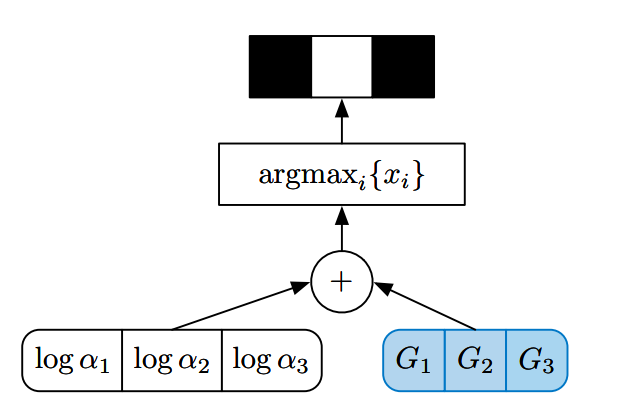
\includegraphics[width=7cm, height=5cm]{gumbel_max}
		\caption{Example of Gumbel-max trick for drawing samples from a discrete distribution whose random variable has 3 states and $\{\alpha_{i}\}_{i=1,2,3}$ as class parameters representing the possibility of occurrence of that class. $\{G_{i}\}_{i=1,2,3}$ are i.i.d Gumbel$(0,1)$ \cite{maddison2016concrete}.}		
		\label{fig:gumbel_max}
	\end{center}
\end{figure}

As observed in Gumbel-Max trick, the sampling step is re-paramterized by one function with distribution parameters and parameter-free random variable as arguments. This function is component-wise addition of two input arguments followed by $argmax$ operation. However, $argmax$ operation is not differential w.r.t. distribution parameter $\alpha_i$. 

With a little abuse of notation, we denote temperature by $\lambda$ here. Fortunately, the $argmax$ operation can be approximated by a continuous function, $softmax$ function with $\lambda$ as temperature parameter, which is differential w.r.t. distribution parameters. With this replacement, we can obtain a continuous approximation to one-hot encoding vector $\bld d$ on the simplex $\triangle^{n-1} = \{\bld x \in \mathbb R^n | x_k \in [0,1], \sum_{i=1}^{n} x_i = 1 \}$:

\begin{equation} \label{gumbel_softmax}
\begin{aligned}
x_{k} = \frac{\text{exp}((\text{log}\alpha_k + G_k)/\lambda)}{\sum_{i=1}^{n}\text{exp}((\text{log}\alpha_i + G_k)/\lambda)}
\end{aligned}
\end{equation}

The sampling steps are similar to Gumbel-Max trick, but with smoothed $softmax$ operation instead of $argmax$(cf. Fig.\ref{fig:gumbel_softmax}). When $\lambda \rightarrow 0$, the $softmax$ function is recovered to $argmax$ operation, when $\lambda \rightarrow \infty$, this operation generates uniform vector instead of one-hot encoding vector. In practice, we set temperature as 0.1.

\begin{figure}[h!]
	\begin{center}
		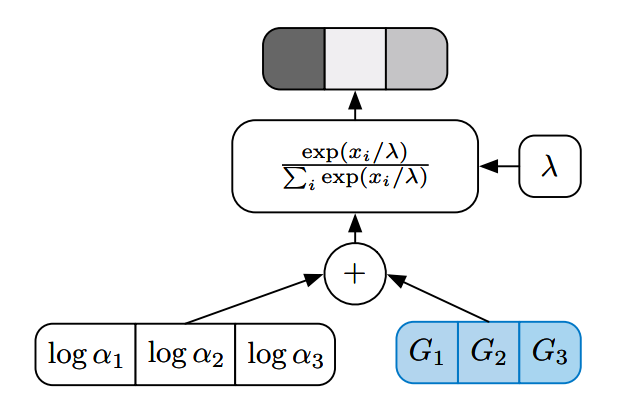
\includegraphics[width=7cm, height=5cm]{gumbel_softmax}
		\caption{Example of continuous approximation to Gumbel-max trick for drawing samples from a discrete distribution whose random variable has 3 states and $\{\alpha_{i}\}_{i=1,2,3}$ as class parameters representing the possibility of occurrence of that class. $\{G_{i}\}_{i=1,2,3}$ are i.i.d Gumbel$(0,1)$\cite{maddison2016concrete}.}		
		\label{fig:gumbel_softmax}
	\end{center}
\end{figure}

When it comes to Bernoulli discrete distribution in our case, it becomes simpler because there are only two states in this distribution and samples live in two dimensional simplex. On the other hand, the difference of two Gumbels distributed random variable is similar to a logistic distributed random variable.  With the probability of state 1 which can be expressed by:

\[
\begin{aligned}
\mathbb P(d_1 = 1) &= \mathbb P(\text{log} \alpha_1 + G_1 >\text{log} \alpha_2 + G_2)\\
&=\mathbb P(\text{log} \alpha_1 - \text{log} \alpha_2 + G_1 - G_2 > 0)
\end{aligned}
\] 

where $G_1 - G_2 = \text{log}(\text{Uniform}(0,1)) - \text{log}(1-\text{Uniform}(0,1))$, which is the inverse cumulative density function of Logistic(0,1).
Then we can infer the re-parameterization of continuous approximation of sample $x \in [0, 1]$ from Bernoulli distributed random variable with $p$ as parameter as follows:

\begin{equation}\label{bern_repa}
\begin{aligned}
x = \text{sigmoid}\big(
\frac{1}{\lambda} (\text{log}p - \text{log}(1-p) + \text{u} - \text{log}(1-u)) 
\big)
\end{aligned}
\end{equation}

where $u \sim \text{Uniform}(0,1)$. 

In order to make explanation more clear and validate the continuous approximate re-parameterization, there is one plot (Fig.\ref{fig:bern_repa}) showing the relationship between average values of 100 samples drawn from this continuous approximation of Bernoulli distribution with different probability parameter from 0 to 1 with step of 0.1. We can see that the empirical average of samples drawn from Eq.\ref{bern_repa} is close to expectation of Bernoulli distribution of corresponding parameter. Additionally, we show one single sample in the figure. As we can see, most of samples are lying on the boundary of range $[0,1]$ and only few of them lie in the interior.
\begin{figure}[h!]
	\begin{center}
		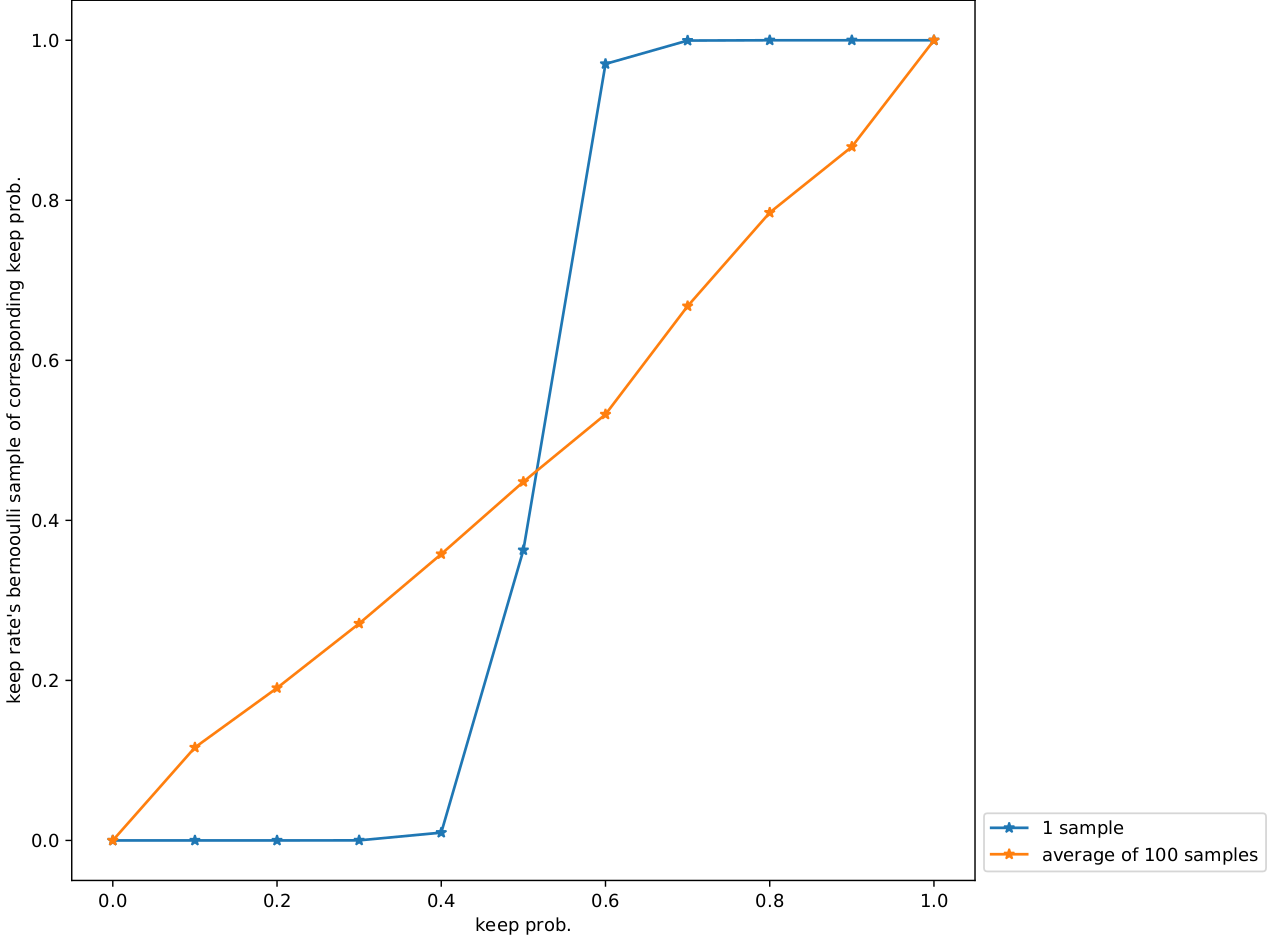
\includegraphics[height=7cm, width=10.5cm]{bern_repa_}
		\caption{One sample and average value of 100 samples drawn from continuous approximation of Bernoulli distribution with parameter $p = [0.1, 0.2, ..., 1.0]$ and temperature $ \lambda =0.1$.}		
		\label{fig:bern_repa}
	\end{center}
\end{figure}

\subparagraph{Dropout regularization:}
Because keep rate of dropout is being optimized, the parameters of approximate distribution $\theta$ contains both $\{ (\bld M_i)_{i=1}^{L} \}$ and $\{(\bld p_i)_{i=1}^{L} \}$. In order to compute gradients of ELBO in Eq.\ref{elbo_grad}, we employ categorical re-parameterization to estimate the gradients w.r.t. Bernoulli distribution parameter $\bld p_i$ in the first term, for the second term, we could not ignore the term with $\bld p_i$ in KL condition Eq.\ref{kl_condition}, which is the entropy term. Consequently, unlike Eq.\ref{KL_grad}, the KL divergence term should be:

\begin{equation} 
\begin{aligned}\label{KL_grad_concrete}
\frac{\partial KL(q_{\theta}(\bld \omega)||p(\bld \omega))}{\partial \theta} 
&\approx \frac{\partial \sum_{i=1}^{L}\lambda||\bld M_{i}||^{2}- \beta\mathcal H(\bld p_{i})}{\partial \theta}  \\
&= \frac{\partial}{\partial \theta} \big( \sum_{i=1}^{L}\lambda||\bld M_{i}||^{2}- \beta D_{i-1}(-p_{i}\text{log}p_{i} - (1-p_{i})\text{log}(1-p_{i}))\big)
\end{aligned}
\end{equation}

where $\lambda$ and $\beta$ are coefficients for L2 regularization and dropout regularization, respectively. They are hyper-parameters which can be tuned based on performance on validation set.
From the equation above, we can see that this term maximize the entropy of Bernoulli distribution, which means this term pushes $\bld p_i$ to 0.5. The coefficient of the dropout regularisation term means that large models will push the dropout probability towards 0.5 much more than smaller models, but as the amount of data N increases the dropout probability will be pushed towards 1 because of the expected log likelihood in the first term. One of reasons behind could be pushing $\bld p_i$ to 0.5 would decrease the capacity of the model which will decrease the expected log-likelihood. 


\subsection{Laplace approximation}
\subsubsection{Introduction}
In this section, another method to approximate the real posterior distribution over weights is introduced, which is called Laplace approximation\cite{bishop2006pattern}. It requires only point estimation of model parameters, thus there is no need to re-train existing model which has already obtained an point estimate. This characteristic makes this approach more appealing  because it's not required to modify the model and thus can be applied to any existing models. The idea behind that is to put a Gaussian approximation on the maximum a posterior point estimate of the model parameters, which is one mode of posterior distribution. The reasons why we consider this method are as following:
\begin{itemize}
	\item it has easy compatibility to existing network. To perform Laplace approximation, we only need one point estimation of model parameters which is already available for most of architectures. That also means, we do not need modify the training phase and we can have approximation of the true posterior for all trained models.
	\item it can capture relationship between model parameters. As mentioned in the first chapter, most of approximation approaches make assumption that parameters are independent to each other for simplicity, scalability as well as computation effort. That could be a quite strong restrictions on the approximation leading to bad performance.
\end{itemize}

In the following, we introduce the basic idea of Laplace approximation and further introduce its scalable version for deep neural network based on Kronecker factor approximation.

Assume we have a point estimate of model parameters via maximum a posterior estimation:
\begin{equation}
\begin{aligned} \label{point estimate}
\bld \omega^\star &= \underset{\bld \omega}{argmax}\{p(\bld \omega|\bld Y,\bld X)\} \\
&= \underset{\bld \omega}{argmax}\{\frac{p(\bld Y|\bld X, \bld \omega) p(\bld \omega)}{p(\bld Y | \bld X)}\} \\
&= \underset{\bld \omega}{argmax}\{p(\bld Y|\bld X, \bld \omega) p(\bld \omega)\}
\end{aligned}
\end{equation}


After taking a second order Taylor expansion of the logarithm of of posterior distribution $p(\bld \omega | \bld Y, \bld X)$ around its mode $\bld \omega^\star$, assuming that the prior of weights is uniform, then we have:

\begin{equation}
\begin{aligned} \label{taylor expansion}
\text{log} p(\bld \omega| \bld Y, \bld X) &\approx 
\text{log}p(\bld \omega^\star|\bld Y, \bld X) + \\
&(\bld \omega - \bld \omega^\star)^T\frac{\partial \text{log} p(\bld \omega| \bld Y, \bld X)}{\partial \bld \omega} + \\
&\frac{1}{2}(\bld \omega - \bld \omega^\star)^T\frac{\partial^2\text{log} p(\bld \omega |\bld Y, \bld X)}{\partial \bld \omega^2}(\bld \omega - \bld \omega^\star)\\
&= \text{log}p(\bld \omega^\star|\bld Y, \bld X) - \frac{1}{2}(\bld \omega - \bld \omega^\star)^T\bld H(\bld \omega - \bld \omega^\star)
\end{aligned}
\end{equation}


where 
\[
\begin{aligned}
\bld H &= -\frac{\partial^2\text{log} p(\bld \omega|\bld Y, \bld X)}{\partial \bld \omega^2}\\
&=-\frac{\partial^2\text{log}\big(p(\bld Y|\bld X, \bld \omega)\big)}{\partial \bld \omega^2} - \frac{\partial^2p(\bld \omega)}{\partial\bld \omega^2}
\end{aligned}
\]

which is negative Hessian of the log posterior. The first order term in Eq.\ref{taylor expansion} vanishes because we expand the function around a local maximum $\bld \omega^\star$, where the first derivative is zero. If we exponentiate this equation, we can get the following Gaussian-like functional form: 

\begin{equation}
\begin{aligned}\label{gaussian form}
p(\bld \omega | \bld Y, \bld X) \propto p(\bld \omega^\star|\bld Y, \bld X)\exp\{-\frac{1}{2}(\bld \omega - \bld \omega^\star)^T\bld H (\bld \omega - \bld \omega^\star)\}
\end{aligned}
\end{equation}

which means $\bld \omega \sim \mathcal N(\bld \omega^\star, \bld H ^{-1})$. Therefore, we can obtain a Gaussian approximate distribution with local maximum $\bld \omega^\star$ as mean and inverse of negative Hessian as covariance matrix.

If we use Gaussian prior for weights. Then it's easy to know that the second order derivative of prior distribution term $\frac{\partial^2p(\bld \omega)}{\partial\bld \omega^2}$ is a identity matrix multiplied by regularization coefficient. And the non-trivial part is the first term, second derivatives of log likelihood. To make the explanation uncluttered, we define the negative Hessian of log likelihood with $\bld{\hat{H}}$ instead:

\[
\bld{\hat{H}} = -\frac{\partial^2\text{log}\big(p(\bld Y|\bld X, \bld \omega)\big)}{\partial \bld \omega^2}
\] 

However, we should note that for a large training set, it's always infeasible to analyze the gradients or Hessian exactly. To resolve this, normally we estimate the expectation of gradients or Hessian in each mini-batch. That means we need to estimate Hessian with empirical average Hessian computed in mini-batches:
\[
\bld{\hat H} \approx N\mathbb E_{p(\bld Y, \bld X)}[\bld{\hat{H}}]
\]
where $N$ is size of training samples, and 
\begin{equation} \label{expected hessian}
\mathbb E_{p(\bld Y, \bld X)}[\bld{\hat{H}}] \approx -\frac{1}{K}\sum_{k}\big[\frac{1}{M}\sum_{i}\frac{\partial^2\text{log}\big(p(y_{ik}|\bld x_{ik}, \bld \omega)\big)}{\partial \bld \omega^2}\big]
\end{equation}

where $K$ is total number of mini-batch, and $(y_{ik}, \bld x_{ik})$ is the $i$-th training data sample in $k$-th mini-batch. 

\paragraph{Fisher information matrix} is an approximation to the expected negative Hessian of exponential family log probability:
\[
\bld{\hat{F}} = \mathbb E_{p(\bld X, \bld Y)}[\bld{\hat{H}}]
\]

Therefore we can use Fisher information matrix as replacement of expected Hessian for the log likelihood term. The derivation of equivalence between expected Hessian and Fisher matrix is straightforward. We define Fisher matrix $\bld F$ in the following:
\begin{equation}
\begin{aligned}\label{Fisher}
\bld{\hat{F}} &= \mathbb E_{p(\bld Y, \bld X)}\big[\frac{\partial}{\partial \bld \omega}\text{log}p(\bld Y|\bld X,\bld \omega)\frac{\partial}{\partial \bld \omega}\text{log}p(\bld Y|\bld X,\bld \omega)^T\big] \\
&\approx \frac{1}{K}\sum_{k}\big[\frac{1}{M}\sum_{i}
\big(\frac{\partial}{\partial \bld \omega}\text{log}p(y_{ik}|\bld x_{ik},\bld \omega)\frac{\partial}{\partial \bld \omega}\text{log}p(y_{ik}|\bld x_{ik},\bld \omega)^T\big)\big]
\end{aligned}
\end{equation}

We include the derivation of equivalence between negative expected Hessian and Fisher matrix for case that parameter is scalar in appendix \ref{appendix:fisher_matrix}, which can be extended to case for vector easily.
Therefore we can obtain 

\begin{equation} \label{fisher hessian}
\bld{\hat{H}} \approx N\bld{\hat{F}}
\end{equation}

and

\begin{equation} \label{fisher hessian_with_prior}
\bld H \approx N\bld{\hat F} + \tau \mathcal {\bld I}
\end{equation}

Actually, computing outer product of gradients requires less computation. But to compute the empirical average of outer product we need to save values with amount quadratic to the number of model parameters inducing large storage overhead. More than that, the computation complexity of inversing matrix is cubic of dimensionality of this matrix which is the number of model parameters. This is also infeasible because the number of parameters in deep neural nets can exceed million easily. Therefore an efficient approximation for Fisher matrix is required. 


\subsubsection{Scalable Laplace approximation for neural network}
In order to mitigate the computational burden in Laplace approximation above, Kronecker-factored approximation curve(KFAC) in \cite{martens2015optimizing} can be used to approximate the Fisher information matrix $\bld F$, with which Laplace approximation can be performed for neural network\cite{ritter2018scalable}. This approximation is derived by approximating the large blocks matrix of Fisher(corresponding to each layer) by Kronecker product of two much smaller matrices. While several times more expensive to compute this, the issues of storage and inversion in Laplace approximation can be mitigated. Additionally, because we need this Fisher information matrix after training, this little expensive computation is required to perform once.

With the notations used in previous subsection, where dropout variational inference is introduced, we will derive the approximation in the following. For clarity, we repeat the definitions of existing notations and new defined ones here. A neural network transforms its input $a_0 = \bld x$ to an output $a_L=p(\bld y| \bld x, \bld \omega)=\sigma(\bld x, \bld \omega)$ through a series of $L$ layers. The units each receive as input a weighted sum of outputs of units from the previous layer and compute their output via a non-linear activation function $\phi(\cdot)$. We denote by $\bld s_i$ the vector of these weighted sums for $i$-th layer, and by $\bld a_i$ the vector output of non-linear activation function. Computation performed for each layer $i\in{1,...,L}$ is given as follows:
\begin{equation}
\bld s_i = \bld a_i\bld W_i \text{ and } \bld a_i = \phi(\bld s_i)
\end{equation}
We define $\bld{\tilde{w}}$ to be the vector consisting of all of the network's parameters concatenated together, i.e. $\bld{\tilde{w}}= \big[vec(\bld W_1)^T \: vec(\bld W_2)^T \: ...\:vec(\bld W_L)^T\big]^T$, where $vec$ is the operator which vectorizes matrices by stacking their columns together. 
For simplicity we first define the following notations:
\[
\partial v = -\frac{\partial \log{p(\bld y, | \bld x \bld \omega)}}{\partial v} \text{ and } \bld g_i = \partial \bld s_i
\]
The first derivatives of objective w.r.t. $\bld{\tilde{w}}$ is defined as follows:
\begin{equation}
\begin{aligned}
\partial \bld{\tilde{w}} = \big[vec(\partial \bld W_1)^T\: vec(\partial \bld W_2)^T\: ...\:vec(\partial \bld W_L)^T\big]^T
\end{aligned}
\end{equation}

From Eq.\ref{Fisher}, we know $\bld{\hat F} = \mathbb E[\partial \bld{\hat w}\partial \bld{\hat w}^T]$ which can viewed as $L$ by $L$ block matrix, with the $(i,j)$-th block $\bld{\hat F}_{i,j}$ given by $\bld{\hat F}_{i,j} = \mathbb E[vec(\partial\bld W_i)vec(\partial\bld W_j)^T]$.

Noting that $\partial \bld W_i = \bld a_{i-1}\bld g_i^T$ and $vec(\bld u \bld v^T) = \bld v \otimes \bld u$, then we have 
\[
vec(\partial \bld W_i) = vec(\bld a_{i-1}\bld g_{i}^T) = \bld g_i \otimes \bld a_{i-1}
\]
Then we can rewrite 
\[
\begin{aligned}
\bld{\hat F}_{i,j} &=  \mathbb E[vec(\partial\bld W_i)vec(\partial\bld W_j)^T]\\
&=\mathbb E[(\bld g_i \otimes \bld a_{i-1})(\bld g_j \otimes \bld a_{j-1})^T]\\
&=\mathbb E[(\bld g_i \otimes \bld a_{i-1})(\bld g_j^T \otimes \bld a_{j-1}^T)]\\
&=\mathbb E[(\bld g_i \bld g_j^T)\otimes(\bld a_{i-1}  \bld a_{j-1}^T)]
\end{aligned}
\]
Here we need to define $\bld{\tilde{F}}_{i,j}$ as approximation to $\bld{\hat F}_{i,j}$ in the following:
\begin{equation}
\begin{aligned}\label{fisher_appr}
\bld{\hat F}_{i,j} &\approx \bld{\tilde{F}}_{i,j} \\
&=\mathbb E[\bld g_i \bld g_j^T] \otimes \mathbb E[\bld a_{i-1} \bld a_{j-1}^T] \\
&= \mathbb E[\bld G_{i,j}] \otimes \mathbb E[\bld A_{i,j}]
\end{aligned}
\end{equation}
where $\bld G_{i,j} = \bld g_i \bld g_j^T$ and $\bld A_{i,j} = \bld a_{i-1}\bld a_{j-1}^T$. The expectation of a Kronecker product is, in general, not equal to the Kronecker product of expectations, and so this
is indeed a major approximation to make, and one which likely won't become exact under any realistic set of assumptions, or as a limiting case in some kind of asymptotic analysis. Nevertheless, it seems to be fairly accurate in practice, and is able to successfully capture the "coarse structure" of the Fisher information Matrix. 
In this work, we only consider the case that layers are independent to others. Therefore the Fisher information matrix of the entire network is a diagonal block matrix, which means $\bld{\tilde{F}}_{i,j}$ is non-zero only for $i=j$. For $i$-th layer, we can compute the Fisher information matrix with Eq.\ref{fisher_appr}. The two factors in Kronecker are outer product of gradients of pre-activation $\bld G_i = \bld g_i \bld g_j^T$ and outer product of activation from previous layer $\bld A_{i} = \bld a_{i-1}\bld a_{i-1}^T$, respectively:
\[
\bld{\tilde{F}}_{i} = \bld G_i \otimes \bld A_i
\] 
If we treat them as covariances of resulting Gaussian. That means each Gaussian has a Kronecker factored covariance, corresponding to a matrix normal distribution\cite{gupta1999matrix}, which considers the two Kronecker factors of the covariance to be the covariances of the rows and columns of a matrix. The two factors are much smaller than the full covariance and allow for significantly more efficient inversion and sampling. The final posterior of Laplace approximation for $i$-th layer is:
\begin{equation}
\begin{aligned} \label{mvg}
\bld W_{i} \sim \mathcal{MN}(\bld W_i^\star, \mathbb E[\bld A_i]^{-1}, \mathbb E[\bld G_i]^{-1})
\end{aligned}
\end{equation}

If we consider Gaussian prior and scale of Fisher information matrix(cf. Eq.\ref{fisher hessian_with_prior}), then the resulting posterior can be written in the following form:

\begin{equation}
\begin{aligned} \label{mvg_prior}
\bld W_{i} \sim \mathcal{MN}(\bld W_i^\star, (\sqrt{N} \mathbb E[\bld A_i]+\sqrt{\tau}\bld I)^{-1}, (\sqrt{N}\mathbb E[\bld G_i]+\sqrt{\tau}\bld I)^{-1})
\end{aligned}
\end{equation} 
where $N$ is the size of training set and $\tau$ is the standard deviation of Gaussian prior.
However, we find that in practice, to treat them as hyper-parameters and tune them w.r.t. the predictive performance on a validation set can yield better performance. The possible reasons for this are two fold. Firstly, nowadays the scale of dataset is really large which can exceed tens of thousand easily. The large size of data could be probably redundant and if we take the redundant data into account and thus increase $N$. This will lead to unreasonably high precision for Gaussian and underestimate the uncertainty significantly. Second, Laplace approximation requires positive definite Hessian and $\tau$ always serves as damp factors to fulfill this condition, therefore it needs to be chosen and tuned carefully.    


\section{Conditional random field}
Graphical models allow us to encode relationships between multiple variables using a concise, well-defined language. Because it's hard to solve the problems deterministically in real world. \textit{Probabilistic graphical model}(PGM)\cite{koller2009probabilistic} can assist in this case by encoding a joint or conditional probability distribution with graph, which means that PGM can encode the relationships between multiple random variables. 

The various types of PGM differ by the graph structure and the conditional independence assumptions. There are mainly two types, directed and undirected graph. Directed graphical model which is also called Bayesian network, specifies the family of distributions by means of directed acyclic graph and its joint distribution is factorized over each node which is a random variable with probability distribution conditioned on its parents. On the other hand, undirected graphical model, also known as Markov random field has undirected acyclic or cyclic graph. Its joint distribution is factorized over cliques, which is a fully-connected subgraph within the graph. This means, the marginal probability distribution in undirected graphical model is not normalized over nodes, but over cliques. 

In a object recognition task, the input is set of images and output is set of predicted labels. Because the dimensionality of input is always large so that it's difficult to model it directly. Nevertheless, we want to exploit the contextual relationship between different objects. To this end, it's better to just model the relationship between output random variables, which obey the conditional distribution of output given input. \textit{Conditional random field}(CRF), first proposed by \cite{lafferty2001conditional}, is a suitable model for this purpose. In this chapter, a concise introduction of CRF is given, including definition, learning and inference in the following subsection.

\subsection{Definition} \label{crf_def}
CRF can model the conditional distribution of a set of output random variables $\bld y$ given a set of inputs $\bld x$, that is $p(\bld y | \bld x)$. In the scope of scene object recognition problem, assume we have multiple objects in one scene denoted by $\bld x = [x_1, ..., x_n]$ and their labels $\bld y = [y_1, ..., y_n]$. We want to learn $p(\bld y | \bld x)$ with CRF and make predictions for unseen data.  

To formulate the problem clearly, we denote the set of output random variables by $\bld y$ and overall output domain by $\mathcal{Y}$. CRF for one scene $\bld x$ is defined by a graph $\mathcal{G} = (\mathcal{V}, \mathcal{E})$, where a set of nodes $\mathcal{V}$ representing the random variables in $\bld y$, and a number of undirected edges $\mathcal{E}\subseteq\mathcal{V}\times\mathcal{V}$ representing the dependencies between random variables. The output domain of CRF is the product of individual variable domains $\mathcal{Y}_i$ so that we have $\mathcal{Y} = \underset{i\in V}{\times} \mathcal{Y}_i$, where $\mathcal{Y}_i = \mathcal{L}$, which is a set of all possible labels. With these notations, we can define the probability distribution of $\bld y$ conditioned $\bld x$ with model parameter $\bld \theta$ as 
\begin{equation}
\label{crf}
\begin{aligned}
p(\bld y|\bld x; \bld \theta) = \frac{1}{Z(\bld x, \bld \theta)}\prod_{c\in\mathcal{C}}\psi_{c}(y_c, x_c, \bld \theta)
\end{aligned}
\end{equation}
where $\mathcal{C}$ is the set of cliques of graph $\mathcal{G}$, and $Z(\cdot)$ is normalizer to make sure $\sum_{\bld y \in \mathcal{Y}}p(\bld y | \bld x; \bld \theta) = 1$, which is also called partition function. $\bld \theta$ stands for the parameters of CRF to be tuned during training phase. $\psi_c(\cdot)$ is called potential function or factor which encodes the contribution of clique $c$ to the total density. The order of number of random variables in clique $c$ can be arbitrary number. However, for computational reason, we only consider factor with number of random variables up to two in normal case. The first order potential is called \textit{unary} potential which means that the clique of this kind of potential contains only one random variable, that is $\psi_i(y_i, x_i, \bld \theta)$. Unary potential can be treated as the likelihood that a label is assigned to this random variable independently to others. The second order potential is called pairwise potential $\psi_{i,j}(y_i,y_j, x_i, x_j, \bld \theta)$ characterized by edges in the graph. This kind of potential states the compatibility of two random variables $(y_i,y_j)$ being assigned to a certain pair of categories. 

To make the explanation more clear, we illustrate a simple example in Fig.\ref{crf}, we ignore $\bld \theta$ here and explain it later and use $\psi_{i,j}$ for $\psi_{i,j}(y_i,y_j,x_i,x_j)$ to make expression of conditional probability uncluttered:

\[
\begin{aligned}
p(y_1, y_2, y_3, y_4) &= \frac{1}{Z(x_1, x_2, x_3, x_4)}\psi_1\psi_2\psi_3\psi_4\psi_{1,4}\psi_{1,2}\psi_{2,3}\psi_{2,3}\psi_{1,2,4} \\
&=\frac{1}{Z(x_1, x_2, x_3, x_4)}\psi_1\psi_2\psi_3\psi_4\psi_{1,4}\psi_{1,2}\psi_{2,3}\psi_{2,3}
\end{aligned}
\]

where the transformation from first line to second line comes from the ignorance of potentials with order higher than two.
\begin{figure}[H]
	\begin{center}
		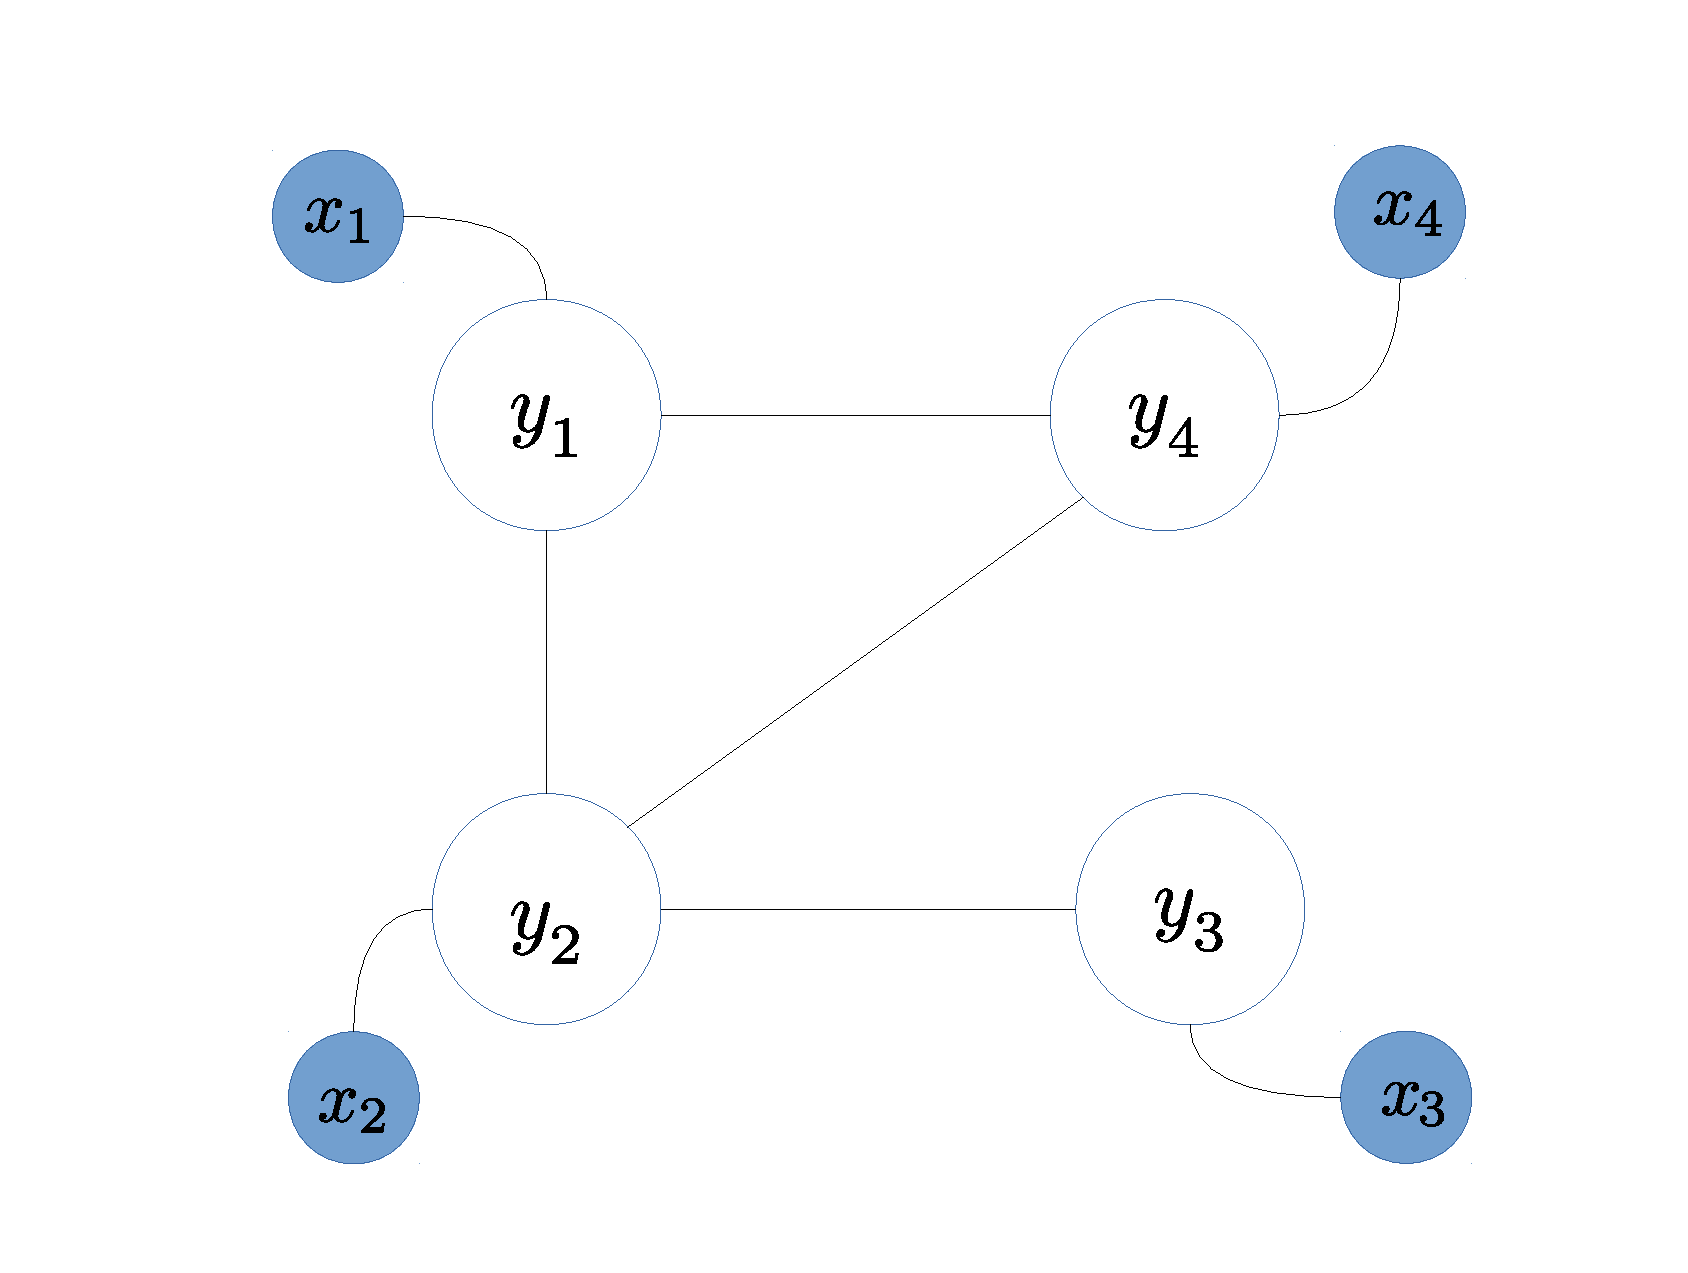
\includegraphics[height=8cm, width=11cm]{crf.eps}
		\caption{Simple example of conditional random field.}		
		\label{crf}
	\end{center}
\end{figure} 
According to Hammersley-Clifford theorem \cite{hammersley1968markov}, the the factors must be always positive, we can employ log-linear models for the potential functions, which results in:
\begin{equation}
\label{crf_potential}
\begin{aligned}
p(\bld y | \bld x; \bld \theta) &= \frac{1}{Z(\bld x, \bld \theta)}\prod_{c\in \mathcal{C}}\exp(\langle\phi(x_c, y_c), \bld \theta\rangle)\\
&=\frac{1}{Z(\bld x, \bld \theta)}\exp(\sum_{i\in V}\langle\phi_u(x_i, y_i), \bld{\theta}_u\rangle + \sum_{(i,j)\in \mathcal{E}}\langle\phi_p(x_i, x_j, y_i, y_j), \bld{\theta}_p\rangle)
\end{aligned}
\end{equation}
being $\langle \cdot, \cdot \rangle$ the inner product, and $\phi(x_c, y_c)$ the sufficient statistic of the factor over clique $c$. Because we consider the potentials up to second order, only feature function for unary potential $\phi_u(\cdot)$ and feature function for pairwise potential $\phi_p(\cdot)$ are considered here. This function can also be treated as feature function which extracts feature of the data over clique. 

Now we have made assumptions of graph structure and conditional dependency for the graph. This can be interpreted as a filter of a probability distribution family. Only the class of probability distribution that satisfies these assumptions such as up to second order potentials can be expressed and learned with this graph. To further identify different probability distribution in this class, we need to parameterize it and identify it with specific parameters which can learned during training. 

\paragraph{Parametrization} of the probability distribution is expressed explicitly in Eq.\ref{crf_potential}. This means that the dimension of the parameter in each kind of potential should be the same as the dimension of feature function. In this work, the feature function should be a function of input and class label, while the feature function can also be the function of only input and weight should be defined as matrix whose output dimension is the number of class serving as a linear mapping. In this work, we only consider the former case.

Regarding \textbf{unary feature}, we utilize the probability vector $p(y_i|x_i)$ which is predictive likelihood from a discriminative classifier which is a deep neural network in this work. 

\paragraph{Pairwise feature} in this work is quite simple context cue in the scene which is defined as binary co-occurrence matrix $\bld H(y_i,y_j)$. If one category occurs with another category in the same scene, then the corresponding entry in the matrix is filled with 1, otherwise 0. 

Although obtaining this pairwise feature requires knowing the ground truth labels of objects in the scene, it still makes sense in the application of this work. Because we use T-LESS dataset which will be introduced in the experiment part, each of scene images in this dataset contains multiple industrial-relevant texture-less objects, some of them are combination of objects of other categories. We want to simulate the situation that, we treat each scene as one product which is composed of multiple sub-parts. Because we know the product, and thus we also know the real labels of components of this product which is corresponding to the co-occurrence of objects in this scene and our goal is to classify the components with help of this contextual information.

Based on these two kinds of features, we have the formulation of likelihood function of CRF model for one scene as follows:
\begin{equation}
\label{crf_used}
p(\bld y|\bld x; \bld \theta) = \frac{1}{Z(\bld x, \bld \theta)}\exp(\theta_u\sum_{i\in V}p(y_i|x_i) + \theta_p\sum_{(i,j)\in \mathcal{E}}\bld H(y_i,y_j))
\end{equation}
where $\bld \theta = \{\theta_u, \theta_p\} \in \mathbb{R}^2$.

\subsection{Learning}
The most popular approach is estimate $\bld \theta$ is maximum likelihood estimate(MLE). The likelihood for one scene is defined in Eq.\ref{crf_used}. Normally we have large size of scenes in training set where each of them contains multiple objects. We denote training set by $\mathcal{D} = [d_1, ..., d_m]$, where each scene is represented by $d_i = (\bld x^i, \bld y^i)$. For each scene, we create a CRF model for it. Therefore we can denote the whole set of graph by $\bld{\mathcal{G}}=[\mathcal{G}_1, ..., \mathcal{G}_m]$, where $\mathcal{G}_i = (V_i, \mathcal{E}_i)$. This is consistent to previous notations when we make little modifications for $\bld x$ and $\bld y$: $\bld x^i = [x^i_1, ..., x^i_n,]$ and $\bld y^i = [y^i_1, ..., y^i_n]$. For computational convenience and stability, negative log likelihood as objective function is always employed. The objective in MLE on training set is defined as fallows:
\begin{equation}
\label{crf_obj}
\mathcal{NLL}(\bld \theta; \mathcal{D}) = -\sum_{i=1}^{m}\big(\theta_u\sum_{j\in V_i} p(y_j^i|x_j^i) + \theta_p\sum_{(j,k)\in\mathcal{E}_i}\bld H(y_j^i, y_k^i)  - Z_l(\bld x^i; \bld \theta)\big)
\end{equation}     
where 
\begin{equation}
\label{log_partition_func}
Z_l = \log
\big(
\sum_{\bld y^i \in \mathcal{Y}} 
\big( 
\theta_u\sum_{j\in V_i}p(y_j^i|x_j^i) + \theta_p\sum_{(j,k)\in \mathcal{E}_i}\bld H(y_j^i, y_k^i) 
\big) 
\big)
\end{equation}

With this expression, our problem is defined in the following form with MLE:
\begin{equation}
\label{crf_nll_opt}
\bld \theta^\star = \underset{{\bld \theta}}{argmin} \big[\mathcal{NLL(\bld \theta; \mathcal{D})}\big]
\end{equation}

The log likelihood function of CRF is proved to be concave \cite{koller2009probabilistic}, which means the local optimizer is also the global optimizer although it's not unique. To optimize this objective w.r.t. the model parameters on dataset with large size, we can employ stochastic gradient descent (SGD), which requires to calculate the gradient of object w.r.t. the model parameters $\bld \theta$. The gradients can be computed as follows, where we use $\bld \theta$ to represent parameters in order to make the expression clear:
\begin{equation}
\label{crf_grad}
\frac{\partial}{\partial \bld \theta} \mathcal{NLL}(\bld \theta; \mathcal{D}) = -\sum_{i=1}^{m}
\big(
\phi(\bld x^i, \bld y^i) - 
\mathbb{E}_{p(\bld y|\bld x^i;\bld \theta)}
\big[\phi(\bld x^i, \bld y)\big]
\big)
\end{equation}
where the expectation $\mathbb{E}_{p(\bld y|\bld x^i;\bld \theta)}
\big[\phi(\bld x^i, \bld y)\big]$ stands for the partial derivative of the log-partition function, which is retrieved by:
\begin{equation}
\label{exp_log_part}
\mathbb{E}_{p(\bld y|\bld x^i;\bld \theta)}
\big[\phi(\bld x^i, \bld y)\big] = \sum_{\bld y\in\mathcal{Y}}p(\bld y|\bld x^i;\bld \theta)\phi(\bld y, \bld x^i)
\end{equation}
The gradients of parameters corresponds to the difference between the empirical expectation of its associated sufficient statistics (the sufficient statistics of ground truth) and its expectation over the estimated probability distribution $p(\bld y|\bld x; \bld \theta)$. The goal of the optimization is to decrease the gradients until they reach zero, which means that we match of first moment of sufficient statistics over the output distribution. Therefore this way is also called moment matching.

When taking a closer look at Eq.\ref{crf_grad} and Eq.\ref{exp_log_part}, to calculate the gradients in each step of SGD, we need to compute $p(\bld y|\bld x; \bld \theta)$, which requires to compute the partition function $Z(\cdot)$. Because the number of possible assignments grows exponentially in the number of classes, it's infeasible to get a exact solution in practice. This problem also appears when we want to obtain a probability distribution(marginal inference) instead of a single prediction(MAP inference) in testing time. To compute the probability distribution in probabilistic modeling always refers to as inference. There are a bunch of research works focusing on inference. Because the CRF model in this work is fully connected, we adopt a popular and effective approach which is called loopy belief propagation and introduced in next subsection. This approach can provide a approximation to the log-partition function $Z_l(\cdot)$, which is required in Eq.\ref{exp_log_part} and to the marginal probability distribution of random variables in $\bld y$ to be plugged in Eq.\ref{crf_grad} in the graph with cycles and exact solution in graph without cycle.


\subsection{Inference}
Loopy belief propagation introduced by \cite{pearl2014probabilistic}, also known as sum-product algorithm, is a popular approach for probabilistic inference in graphical models. Briefly, this approach is based on the exchange of statistical information among the nodes in the graph according to their relationships. The core idea behind that is for each node in the graph to maintain its belief, which is a $k$-dimensional vector $\bld b(y_i)$ if the node is discrete random variable where $k$ is the number of class. The $i$-th entry of this vector indicates the probability that $i$-th class is assigned to this node. The belief of a node evolves as it receives \textit{messages} from it neighbors. A message $\bld m_{ij}(y_j)$ sent from node $y_i$ to node $y_j$ encodes belief of $y_i$ about what class node $y_j$ should belong to. This message, in turn, based on the messages it received from all the other neighbors except for the recipient in a previous time-step.

The algorithm keeps sending messages until the graph is calibrated, which means that the messages of two consecutive iterations are less than one threshold. However, in practice, the algorithm can not calibrate or converge. A maximum number of iteration can be set to obtain satisfactory results. The messages computation is as follows:
\begin{equation}
\label{message}
\bld m_{ij}(y_j) = \sum_{y_i\in \mathcal{Y}_i}\psi_{ij}(y_i, y_j, x_i, x_j, \theta_p)\psi_i(y_i, x_i, \theta_u) \prod_{y_k\in\mathcal{N}(y_i)\backslash y_j}\bld m_{ki}(y_i)
\end{equation}
where $\mathcal{N}(y_i) \backslash y_j$ is the set of node neighbors of $y_i$ except for $y_j$. Once the iteration reaches maximum number or the graph is calibrated, we can compute the belief of each node as follows:

\begin{equation}
\label{belief}
\bld b(y_i) = \frac{1}{Z_i}\psi_i(y_i, x_i, \theta_u) \prod_{y_j\in\mathcal{N}(y_i)}\bld m_{ji}(y_i)
\end{equation}
where $Z_i$ is the normalizer of unnormalized belief of node $y_i$ to ensure the sum of marginal probability of $y_i$ is 1. 


